When studying something like viruses, that can have a huge effect on a person let alone a society, it is crucial to produce accurate simulations quickly. In the previous chapter, I showed how the field of virology has tried to use ABMs to capture the spatial spread of viruses, but does not have either the computing power or coding tools to make the ABMs feasible. In this chapter, a model for studying virus that incorporates the physics of viral spread both quickly and accurately is given in detail. I will present how the model accounts for spatial spread of virus, is able to produce simulations without compromising on accuracy, and can be applied to real experimental data. 

\section{Model details}

In this work, a two dimensional biological system is simulated with a mathematical model. The system is a culture dish of a monolayer of cells with virus diffusing over the cells. The model is a hybrid of an agent based model (ABM) and a partial differential equation model (PDM) where the cells are represented with an ABM and the virus diffusion is represented by a PDM.

\subsection{Spatial accounting} \label{Spatial_accounting}

To allow for the two dimensional aspect of the culture dish to be represented in the model, the cells are approximated as hexagons. Using hexagons enables for an elegant managing of the cells' shapes in the dish and the viral transmission. Since the culture dishes are grown to confluence, the cells are close enough that they push on each other and the cell walls deform. This causes the cells to no longer be in the shape of a circle, but become irregular polygons with multiple sides \citep{bruckner_importance_2018}. Modeling the cells as hexagons gives the cells definite sides and the cells are able to span any two dimensional region forming a hexagonal grid. Furthermore, by using a hexagonal grid, when virus particles spread among this population of cells the indexing of the grid can be used to find the neighbors of any cell. This will be used for cell-free transmission to know where virus will flow away from (high concentrations areas) and to (low concentration areas) during diffusion. In addition to helping with the physical representation of the model, hexagonal coordinates have some other attributes that can be utilized to optimize the code for quicker compute times. The three attributes that this code utilizes are:
\begin{enumerate} 
    \item The coordinates can be split in to three sectors where the coordinates $X_{hex}$, $Y_{hex}$, and $Z_{hex}$ are simply cyclic permutations.
    \item The $X_{hex}$ and $Z_{hex}$ directions can be used as indices of a matrix.
    \item The coordinates of the neighboring hexagons are found by adding a cyclic permutation of 
        $\left [
            \begin{array}{c}
                1 \\
                0 \\
                -1\\
            \end{array}
        \right ]$
        for three of the neighbors and
        $\left [ 
            \begin{array}{c}
                1 \\
                -1 \\
                0\\
            \end{array}
        \right ]$
        for the other three neighbors.
\end{enumerate}
These attributes save time by either reducing the number of calculations needed or the amount of searching through data arrays. Attribute 1 allows for only a third of the cell locations to be calculated and Attributes 2 and 3 give the data a reference so that adjacent data in memory can be found quicker.

\subsection{Agent-based model} \label{ABM}

In an ABM, a system is broken down into smaller units called ``agents''. Each of the agents are governed by a set of rules on a local scale with large scale phenomena resulting from interaction of the agents, so the two scales are studied to find the connections. As a simulation of the model is stepped through time, the agents act and interact. These actions cause bulk properties, that may appear disconnected from the individual agents, to manifest. Properties are observed and measured to find the connection between the small interactions and large scale properties.

In this work, an ABM governs the transitions a cell makes through the stages of infection: healthy, eclipse, infected, and dead. A cell in the healthy state is an uninfected cell that remains healthy until infected. A cell in the eclipse state is an infected cell that is not yet producing virus. The cell remains in the eclipse state for an average amount of time, $\tau_E$. The specific time value for each cell is determined by a gamma distribution with shape value $\eta_E$ and scale value $\tau_E/\eta_E$. A cell in the infected state is an infected cell that is producing virus. The cell remains in the infected state for an average amount of time, $\tau_I$. The specific time value for each cell is determined by a gamma distribution with shape value $\eta_I$ and scale value $\tau_I/\eta_I$. A gamma (Erlang) distribution is used for the amount of time in the eclipse and infected phase, as suggested by the work of Beauchemin et al.\ \citep{beauchemin17} and Kakizoe et al.\ \citep{kakizoe15}. A cell in the dead state is a cell that can no longer change state, so once a cell is in the dead state the cell remains in that state until the end of the simulation. The flow of this is illustrated in figure \ref{fig:transitioning_through_the_stages_of_infection}.

The ABM uses four time arrays to track and transition the cells to different states after infection. The four arrays universal time (UT), healthy time (HT), eclipse time (ET), and infected time (IT) have an element for each cell. The universal time array holds the amount of time that each cell has been in the simulation; each element starts at zero and increases each iteration by the simulation's time step. The healthy time array holds the amount of time that a cell is healthy; each element starts at zero and while the cell is healthy increases each iteration by the simulation's time step. The eclipse time array holds the amount of time each cell is in the eclipse state and the infected time array holds the amount of time each cell is in the infected state. For the eclipse and infected arrays the amount of time is fixed and the value is determined by a gamma (Erlang) distribution, as described above. The flow of this is illustrated in figure \ref{fig:transitioning_through_the_stages_of_infection}.

%\begin{figure}
%    \centering
%    \begin{tikzpicture}[state/.style={regular polygon,regular polygon sides=6, draw, minimum size=2.5cm, inner sep=0pt, outer sep=0pt}]
%    \node[state, draw=AGreen, fill=AGreen!10] (H) {$Healthy$};
%    \node[state, draw=cyan, fill=cyan!10, right of=H] (E) {$Eclipse$};
%    \node[state, draw=red, fill=red!10, right of=E] (I) {$Infected$};
%    \node[state, draw=black, fill=black!10, accepting, right of=I] (D) {$Dead$};
%    
%    \draw   (H) edge[bend left=45] node [above] {} (E);
%    \draw   (E) edge[bend left=45] node [above] {$\tau_E$} (I);
%    \draw   (I) edge[bend left=45] node [above] {$\tau_I$} (D);
%    \end{tikzpicture}
%    \caption{The stages of infection healthy, eclipse, infected, and dead are shown. Cells stay in  the eclipse stage for an average time $\tau_E$ and in the infected stage for an average time $\tau_I$.}
%    \label{fig:stages_of_infection}
%\end{figure}

%\begin{figure}
%    \centering
%    \begin{tikzpicture}[state/.style={regular polygon,regular polygon sides=6, draw, minimum size=2.5cm, inner sep=0pt, outer sep=0pt}]
%        \node[state, draw=AGreen, fill=AGreen!10] (H) {$Healthy$};
%        \node[state, draw=cyan, fill=cyan!10, below right of=H] (E) {$Eclipse$};
%        \node[state, draw=red, fill=red!10, below right of=E] (I) {$Infected$};
%        \node[state, draw=black, fill=black!10, accepting, below right of=I] (D) {$Dead$};
%            
%        \draw   (H) edge[bend left=45] node [above right] {Infection event} (E);
%        \draw   (E) edge[bend left=45] node [above right] {UT $>$ HT + ET} (I);
%        \draw   (I) edge[bend left=45] node [above right] {UT $>$ HT + ET + IT} (D);
%    \end{tikzpicture}
%    \caption{Transitioning through the stages of infection: UT is the universal time for a cell, HT is the healthy time for a cell, ET is the eclipse time for a cell, and IT is the infected time for a cell.}
%    \label{fig:transitioning_through_the_stages_of_infection}
%\end{figure}

\begin{figure}
    \centering
    \begin{tikzpicture}[
        Healthy/.style={regular polygon,regular polygon sides=6, draw, minimum size=2.5cm, inner sep=0pt, outer sep=0pt, draw=AGreen, fill=AGreen!10},
        Eclipse/.style={regular polygon,regular polygon sides=6, draw, minimum size=2.5cm, inner sep=0pt, outer sep=0pt, draw=cyan, fill=cyan!10},
        Infected/.style={regular polygon,regular polygon sides=6, draw, minimum size=2.5cm, inner sep=0pt, outer sep=0pt, draw=red, fill=red!10},
        Dead/.style={regular polygon,regular polygon sides=6, draw, minimum size=2.5cm, inner sep=0pt, outer sep=0pt, draw=black, fill=black!10}]

        \node[Healthy] (H) {$Healthy$};
        \node[Eclipse, below right of=H] (E) {$Eclipse$};
        \node[Infected, below right of=E] (I) {$Infected$};
        \node[Dead, accepting, below right of=I] (D) {$Dead$};
            
        \draw   (H) edge[bend left=45] node [above right] {Infection event} (E);
        \draw   (E) edge[bend left=45] node [above right] {UT $>$ HT + ET} (I);
        \draw   (I) edge[bend left=45] node [above right] {UT $>$ HT + ET + IT} (D);

        \draw   (H) edge[bend right=45] node [below left] {} (E);
        \draw   (E) edge[bend right=45] node [below left] {$\tau_E$} (I);
        \draw   (I) edge[bend right=45] node [below left] {$\tau_I$} (D);

        %Legand with text
        \matrix [draw,
                below right,
                column 1/.style={anchor=base west},
                column 2/.style={anchor=base west}
                ] at (current bounding box.north east) 
        {
          \node [] {UT}; & \node [] {Universal time}; \\ 
          \node [] {HT}; & \node [] {Healthy time}; \\ 
          \node [] {ET}; & \node [] {Eclipse time}; \\ 
          \node [] {IT}; & \node [] {Infected time}; \\ 
        };

%        %Legand with nodes
%        \matrix [draw, below left] at (current bounding box.north east) {
%          \node [Healthy, scale=0.3, label=right:Healthy] {}; \\
%          \node [Eclipse, scale=0.3, label=right:Eclipse] {}; \\
%          \node [Infected, scale=0.3, label=right:Infected] {}; \\
%          \node [Dead, scale=0.3, label=right:Dead] {}; \\
%        };
    \end{tikzpicture}
\caption{The stages of infection: healthy, eclipse, infected, and dead are shown. The cells transition through the stages at different time points. Above: The time point when a state transition occurs is shown in terms of UT, the universal time, for a cell. Below: The time point when a state transition occurs is shown in terms of average time. $\tau_E$ is the average time a cell stays in  the eclipse stage and $\tau_I$ is the average time a cell stays in the infected stage. UT is the time a cell has existed, HT is the time a cell has been healthy, ET is the time a cell is in the eclipse phase, and IT is the time a cell is in the infected phase. \label{fig:transitioning_through_the_stages_of_infection}}
\end{figure}

\subsection{Partial differential equation model} \label{PDM}

PDMs are used to model multiple dimensions; in this work a PDE in hexagonal coordinates is used to model the two-dimensional spatial spread of virus over cells in a culture dish. In a PDM, the dynamics of a system can be represented by a partial differential equation, or more specifically, an equation that contains multi-variable functions that represent important system aspects and one or more partial derivatives of those functions. In the culture dish, as an infected cell releases virus into the extracellular fluid, the virus diffuses across a density gradient. The PDM represents this diffusion with the diffusion equation, 
\begin{equation}
\frac{\partial V}{\partial t}=D \nabla^{2}V + p - cV, \label{diff_eq}
\end{equation}
where $V$ is the density of the virus, $D$ the diffusion coefficient, $p$ is the production rate per cell, $c$ is the viral clearance rate. In the code, along with the assumption of hexagonal cells, the cells are assumed to be flat, so the virus is diffusing over a smooth two dimensional plane. This assumption allows for the use of the two dimensional diffusion equation in hexagonal coordinates, so Eq.\ \eqref{diff_eq} becomes 
$$\frac{\partial V}{\partial t} = D\frac{2}{3} \left (\frac{\partial^2}{\partial x^2_1}+\frac{\partial^2}{\partial x^2_2}+\frac{\partial^2}{\partial x^2_3}\right )V + p -cV$$ 
where  
$\textbf{x}_1=
\left [
    \begin{array}{c}
        1 \\
        0 \\
    \end{array}
\right ]$, 
$\textbf{x}_2=
\left [
    \begin{array}{c}
        -1/2 \\
        \sqrt{3}/2 \\
    \end{array}
\right ]$, and 
$\textbf{x}_3=
\left [
    \begin{array}{c}
        -1/2 \\
        -\sqrt{3}/2 \\
    \end{array}
\right ]$ 

are the unit vectors for a hexagonal grid. For computation, a forward Euler implementation of the PDM with Neumann boundary conditions is used.

\subsection{Viral transmission} \label{Viral_transmission}

When a virus is spreading among the cells in a culture dish, there is a probability that a healthy cell becomes infected by virus that is not within a cell, but flowing around and above the cell. When this viral transmission occurs it is called cell-free transmission. For cell-free transmission, the probability per unit time ($\mathrm{P_{cf}}$) that a cell becomes infected is determined by the amount of virus that is covering the cell ($V$) times the infection rate ($\beta$) \citep{holder11autoimm}, 
$$\mathrm{P_{cf}} = V \beta.$$ 
As a healthy cell becomes surrounded by more virus, the probability of cell-free infection increases. If the probability ($V \beta \Delta t$) is ever greater than one due to the build up of virus, an adaptive time step is used. The time step ($\Delta t$) is divided in half repeatedly until the probability of cell-free infection is below one. Once the probability is finalized, a number from the uniform distribution is compared with the probability of cell-free infection. If that number is less than $\mathrm{P_{cf}}$, then the cell becomes infected.

%1 - y = (1-m)^n

\subsection{Parameters of viral spread}

The eight parameters $\beta$, $\tau_E$, $\eta_E$, $\tau_I$, $\eta_I$, $p$, $c$, and $D$ affect the dynamics of virus spread in the model. Four of the parameters, $\tau_E$, $\eta_E$, $\tau_I$, and $\eta_I$, are used in the ABM to choose the time duration that a cell is in the eclipse and infected phase as mentioned in section \ref{ABM}. Three of the other parameters, $p$, $c$, and $D$, are used in the PDM and characterize the differential equation, as mentioned in section \ref{PDM}. The final parameter, $\beta$, governs the interaction between the virus and cells, setting the probability that the cell is infected. In order to model a particular virus, values for these parameters need to be chosen. The initial values of the parameters are chosen from ordinary differential equation models of influenza and listed in Table \ref{tab_params} (viral titer units have been converted to virions, as described in \citep{dobrovolny17}). %For $\eta_E$, $\eta_I$, $c$, and $D$ the values are fixed, but for $\beta$, $\tau_E$, $\tau_I$, and $p$ the values serve as a starting point for the model to be fit to real experimental data.

\begin{table}
%\centering
\caption{Parameter values to simulate an influenza infection with the ABM/PDM model.\label{tab_params}}
\resizebox{\textwidth}{!}{%
\begin{tabular}{llcr}
\hline
Parameter & Meaning & Value & Reference\\
\hline
$\beta$ & Infection rate & 2.0 $/\mathrm{h}$ & Scaled from Beauchemin et al.\ \citep{beauchemin08}\\
$p$ & Viral production rate & 562800 $/\mathrm{h}$ & Scaled from Beauchemin et al.\ \citep{beauchemin08}\\
$c$ & Viral clearance rate & 0.105 $/\mathrm{h}$ & Beauchemin et al.\ \citep{beauchemin08}\\
$D$ & Diffusion coefficient & 2.16$\times 10^{-8}$ $\mathrm{m}^2/\mathrm{h}$ & Stokes-Einstein equation\\
$\tau_E$ & Mean eclipse duration & 6.0 $\mathrm{h}$ & Beauchemin et al.\ \citep{beauchemin08}\\
$\eta_E$ & Eclipse shape parameter & 30 & Pinilla et al.\ \citep{pinilla12}\\
$\tau_I$ & Mean infectious lifespan & 12.0 $\mathrm{h}$ & Beauchemin et al.\ \citep{beauchemin08}\\
$\eta_I$ & Infectious shape parameter & 100 & Pinilla et al.\ \citep{pinilla12}\\
\end{tabular}}
\end{table}

%In order to determine which parameter values minimize the SSR, a brute force walk of a parameter space is performed. The axes of the parameter space are four arrays that are constructed around the initial values of $\beta$, $p$, $\tau_I$, and $\tau_E$, shown in Table \ref{tab_params}. Two values, increasing or decreasing by 25\%, are added on both sides of the initial points; resulting in a total of 5 points per array and 625 points total in the parameter space.

\section{Computational details}

In this work, the simulations are of viral infections, that can have drastic effects on those infected, so the model needs to produce simulations that are fast, numerically sound, and have realistic results. The model uses parallel processing on GPUs to reduce simulation times without reducing complexity. Additionally, the simulations are tested for numerical convergence and are then fit to real experimental data in order to reproduce experiments.

\subsection{Implementation on GPUs}

As the model becomes more complex, GPU acceleration via parallel programming is used to decrease the simulation run times and therefore increase the number of studies that can be conducted in a given time. In the simulations, the cells change state based on the amount of virus above them. The number of cells in a culture dish is on the order of $10^6$ cells \citep{Number_of_cells_in_a_dish_noauthor_useful_nodate}, so the ABM will simulate a grid of $1001365$ agents of hexagonal cells in a circle to best replicate what is happening in the experiment. Each agent will follow the rules of checking the amount of virus above the cell every time step. Utilizing attribute 2 of hexagonal coordinates from section \label{Spatial_accounting}, the number of calculations is reduced from the order of ($\mathcal{O}(n^2)$) per time step to the order of the number of agents ($\mathcal{O}(n)$). The calculations from the agents' rules are split over the processing units of a GPU to be calculated in parallel or simultaneously. To utilize this processing, Nvidia's CUDA (Compute Unified Device Architecture) is used to implement the ABM and PDM. CUDA is an Application Programming Interface (API) that allows the many processing units (cores) on a Nvidia brand GPU to be used for computing. %The ability to manipulate what is happening at the cellular level of the simulations allows for generation of isolated studies of the viral transmission. The isolated studies of how cells are infected are analyzed and the characteristics from section \ref{Viral_transmission} are compare to find any trends in the data



%%%%%%%%%%%%%%%%%%%%%%%%%%%%%%%%%%%%%%%%%%%%%%%%%%%%%%%%%%%%%%%%%%%%%%%%%%%%%%%%%%
\subsection{Convergence Testing} \label{methods_convergance}

Partial differential equations (PDEs) are a popular way to model systems that evolve over both space and time, but often require computers to produce solutions. With PDEs, even systems that have an exact solution often need to be calculated on a computer because of the infinite series that are required in those solutions. Therefore, solutions to PDEs are often found through numerical integration. In the numerical integration, space and time are assumed to be made up of small units or discretized. From this discretization, time is a one dimensional line of points separated by a chunk of time called $\Delta t$ and two dimensional Cartesian space is a grid with a line of points for each dimension where there is a chunk of space for each dimension $\Delta x$, $\Delta y$. At these points in time and space, a numerical integration scheme approximates the solution of the PDE. Different numerical schemes have different benefits. Depending on the phenomena that needs to be studied with the PDE the size of $\Delta t$, $\Delta x$, and $\Delta y$ and the choice of numerical scheme are important. If the chunks of space or time are too large then the simulation does not have the resolution to resolve phenomena that occur at smaller increments in the model and if the numerical scheme requires to much computing power then the solutions can not be found in a timely manner.

Depending on the choice of numerical scheme, a conditional relationship between $\Delta t$, $\Delta x$, and $\Delta y$ must be met. For the symmetric, two dimensional Euler's method $$ \Delta t \leq \frac{(\Delta x)^{2}}{4 D},$$ is the conditional relationship \citep{wendroff_difference_1968,olsen-kettle_numerical_nodate}. Satisfying this relationship is necessary to ensure that the sequence of approximations that the numerical scheme uses to approximate a solution converges, otherwise the error grows exponentially to a point that the solutions are unreliable. Using the relationship above, values for $\Delta t$, $\Delta x$, and $\Delta y$ can be chosen to ensure stability of the error in the numerical scheme. As long as that relationship is met the solution is reliable within a certain error, but the relationship does not give the $\Delta t$, $\Delta x$, and $\Delta y$ that are best for producing accurate simulations with the least amount of computing cost.

To ensure the simulations are not using more resources than necessary, the space and time discretizations: $\Delta t$, $\Delta x$, and $\Delta y$ need to be optimized. Convergence testing is a simple brute force method where the input parameters are increased or decreased by a particular amount and the accuracy or trends of the simulation are measured for each of the the new increments. Schemes for convergence testing are implemented and studied in fields like computational fluid dynamics \citep{bermejo16,kim20fluid} and astrophysics \citep{xu21,banei21}. The model proposed in this work has fixed $\Delta x$ and $\Delta y$, because the simulations are of real cells, whose average diameter can be measured between \numrange[range-phrase = --]{50}{100} \si{\micro\meter}. Thus the convergence testing only has to be conducted for $\Delta t$. To conduct the study a starting point of 0.005 hr, about 5.78 times smaller than the conditional relationship, was chosen and a range of seven values was created by multiplying or dividing the initial $\Delta t$ by 2 repeatedly. For each of these $\Delta t$s, the median viral titer curve of ten simulations were compared.

\subsection{Measurements} \label{convergence_measures}

As the viral infection progresses the total amount of virus in the culture dish changes and the shape of the total amount of virus over time can change depending on the virus being use for the infection. Plotting the amount of virus vs.\ time produces a curve that has a distinct shape and has characteristics that can be measured. The measurements, shown in Figure \ref{measurements} and definitions listed below, can be used to compare multiple viruses or to compare multiple simulations of the same virus with different input parameters. In this thesis, I will use them to verify the convergence of the simulation.
\begin{itemize}
\item \textbf{peak viral load:} The maximum amount of virus is commonly used as an indicator of the transmissibility of an infection \citep{handel09}. 
\item \textbf{time of viral peak:} This is the time between the start of the infection and the peak of the virus and can give an indication of how quickly the virus is replicating.
\item \textbf{viral upslope:} Viral upslope is the exponential growth rate of the viral titer before the peak is reached and is another indication of how quickly the virus is spreading from cell to cell. 
\item \textbf{viral downslope:} Viral downslope is the exponential decay rate of the viral titer after the peak. While the slope during the decay phase is negative, we define downslope as the positive value of the slope.
\item \textbf{area under the curve (AUC):} AUC is often used to assess the severity of an infection \citep{hayden00, barroso05}.
\item \textbf{infection duration:} The infection duration is indicative of how long an infected patient might test positive for presence of the virus. In this work $10^1$ virions is the threshold.
\end{itemize}

\begin{figure}
\begin{center}
    \resizebox{0.6\textwidth}{!}{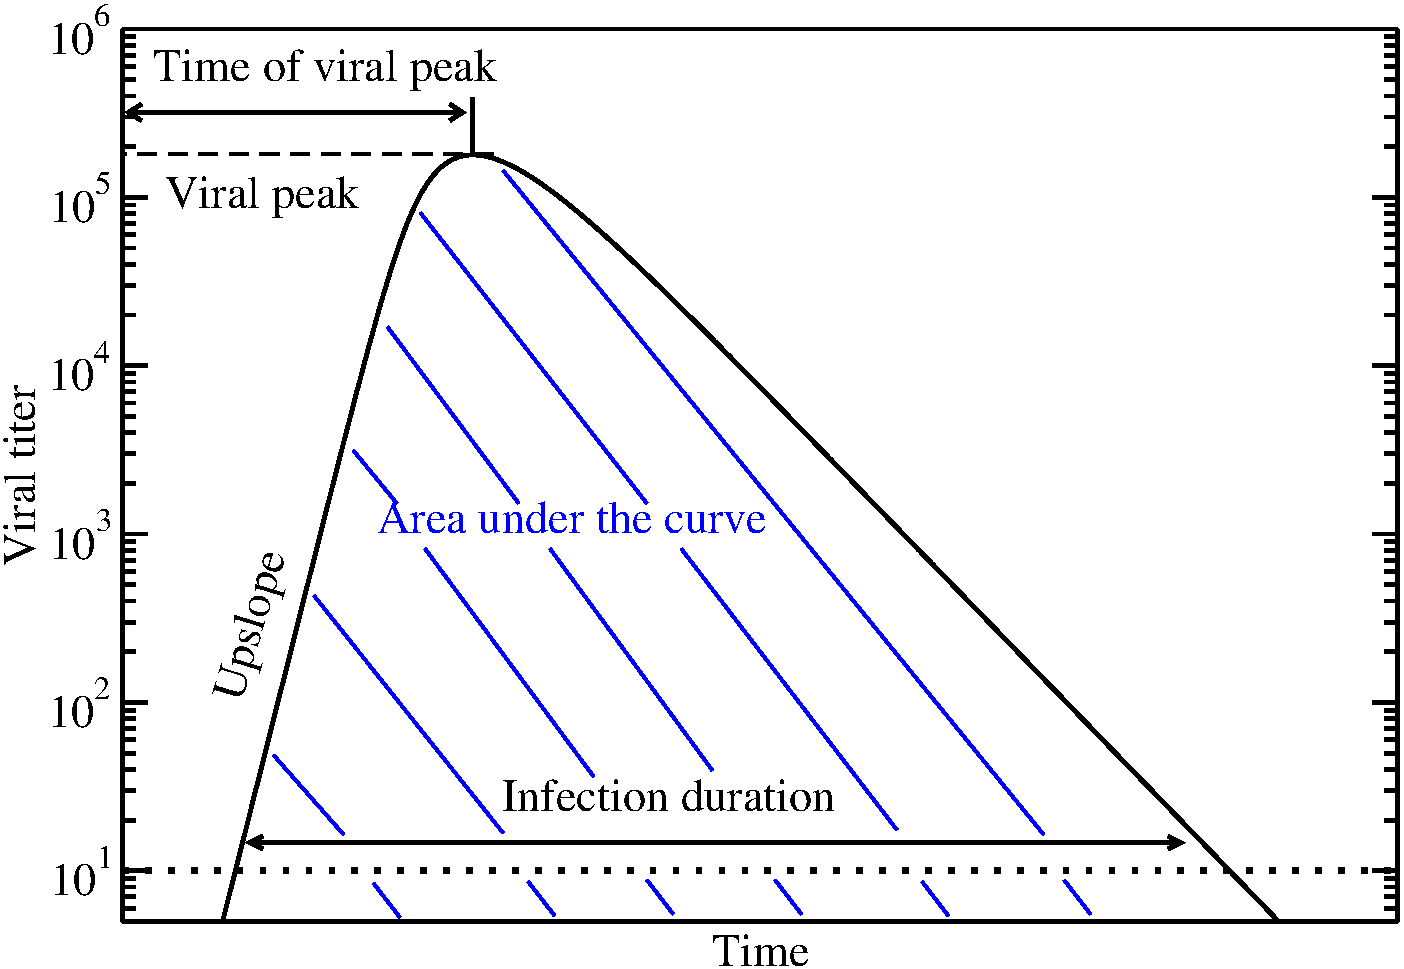
\includegraphics{Figures/measurements.pdf}}
    \caption{Measurable characteristics of the viral titer curve.}
    \label{measurements}
\end{center}
\end{figure}


\section{Data Fitting} \label{Data_Fitting}

As part of our model validation, the model is tested to ensure it can reproduce viral titer curves observed experimentally. We use three experimental data sets varying both virus and cell type. The first data set used here is from an \emph{in vitro} experiment performed by Pinilla et al.\ \citep{pinilla12}. During the study, a well of a 24-well plate, containing Madin-Darby canine kidney (MDCK$\alpha$2,6) cells was inoculated with the A/Qu\'{e}bec/144147/09 (H1N1) pandemic strain of influenza virus and the supernatant fluid was collected every 6 hours until 36 hours and then every 12 hours until 72 hours post infection. The supernatant was then used for RNA isolation and/or viral titration by standard plaque assay on MDCK$\alpha$2,6 cells. The specific data referenced for this work is the ``Multiple-cycle viral yield" experiment shown in figure 2A of the Pinilla et al.\ manuscript. The second and third data sets are from an \emph{in vitro} experiment performed by Wang et al.\ \citep{wang_susceptibility_2021}. The Vero and Vero76 cell lines will be used for the fitting process. During the study, 25 cell lines where inoculated with \num{5e4} TCID$_{50}$ per well of  SARS-CoV-2/USA-WA1/2020 (USA-WA1). The supernatant fluid was recorded initially at 0 hours, then collected at 2 hours, then, from 0, collected every 24 hours until 120 hours post infection. The supernatant was then used for viral RNA quantification. The specific data referenced for this work is the Vero cell lines and the Vero76 cell lines of the ``Replication of SARS-CoV-2 in a Large Set of Cell Substrates" experiment shown in figure 2 of the Wang et al.\ manuscript. 

To determine the best fit of the model to the experimental data, the sum of square residuals (SSR) is minimized, $$\mathrm{SSR} = \sum_{i=1}^{n} (y_i - \hat y_i)^{2},$$ where $y_i$ is from the experimental data set and $\hat y_i$ is from the simulated data set. In our case, the simulated data set is the average of ten cell-free transmission simulations. The initial conditions for the simulations are: Total cells -- $1001365$, Total virus -- $0.0$, and MOI -- $5\times 10^{-5}$. To perform the minimization, a separate code that utilizes the function \texttt{minimize} from the python package \texttt{scipy}, was written. In the code, five parameters ($\beta$, $p$, $\tau_I$, $\tau_E$, and $c$) are allowed to vary and the remaining parameters are held fixed to the values given in Table \ref{tab_params}. The minimization code is given an initial guess for the five parameters, then by the Nelder-Mead method the next set of parameters is produced, until the minimum SSR is found.
%%%%%%%%%%%%%%%%%%%%%%%%%%%%%%%%%%%%%%%%%%%%%%%%%%%%%%%%%%%%%%%%%%%%%%%%%%%%%%%%%%%

\section{Summary}

In this chapter, I've described the construction of a hybrid ABM/PDM model of viral infections and I've outlined the techniques that will be used to test the reliability and validity of the model. 
